% ====================================================================
% VİZE RAPOR ŞABLONU – Türk Masalları Derlemesi Web Sayfası
% --------------------------------------------------------------------
% DERLEME: Overleaf'te Menu > Compiler > XeLaTeX (pdfLaTeX de çalışır).
%
% KURALLAR (şablonu kullanmadan önce okuyun):
%  1. Bölüm başlıklarını SİLMEYİN ve sırasını DEĞİŞTİRMEYİN.
%  2. [KÖŞELİ PARANTEZ] içindeki ve gri renkli açıklama metinlerini
%     kendi bilgilerinizle değiştirin; açıklama metinlerini silin.
%  3. MEBİS'e YALNIZCA bu raporun PDF'ini yükleyin.
%     ZIP ve HTML dosyası YÜKLEMEYİN. Tüm kontroller GitHub'dan yapılır.
%  4. Kapaktaki GitHub ve YouTube bağlantıları doğru ve tıklanabilir
%     olmalıdır. Teslimden önce PDF'teki bağlantılara tıklayıp deneyin.
%  5. Haftalık katkı tablosundaki görseller için resim dosyalarını
%     (hafta1.png, hafta2.png, ...) Overleaf projesine yükleyin.
%     Dosya adlarında boşluk ve Türkçe karakter kullanmayın.
%     Resim yoksa tabloda "görsel ekleyin" kutusu görünür.
%  6. Yapay zekâ kullandıysanız Bölüm 5'i doldurun.
% ====================================================================
\documentclass[12pt,a4paper]{article}

\usepackage{iftex}
\ifPDFTeX
  \usepackage[T1]{fontenc}
  \usepackage[utf8]{inputenc}
\else
  \usepackage{fontspec}
\fi
\usepackage[turkish]{babel}
\usepackage[margin=2.4cm]{geometry}
\usepackage{setspace}
\usepackage{graphicx}
\usepackage{booktabs}
\usepackage{longtable}
\usepackage{array}
\usepackage{colortbl}
\usepackage{xcolor}
\usepackage{enumitem}
\usepackage{listings}
\usepackage{amssymb}
\usepackage{caption}
\usepackage{fancyhdr}
\usepackage{hyperref}

\onehalfspacing
\setlength{\parindent}{0pt}
\setlength{\parskip}{6pt}
\setlist{itemsep=2pt, topsep=4pt}
\hypersetup{colorlinks=true, linkcolor=blue!50!black, urlcolor=blue!50!black}

\definecolor{ana}{HTML}{14325C}
\definecolor{acik}{HTML}{EEF2F8}

\lstset{basicstyle=\ttfamily\small, backgroundcolor=\color{acik},
  frame=single, rulecolor=\color{ana}, breaklines=true,
  columns=fullflexible, keepspaces=true, showstringspaces=false}

\pagestyle{fancy}
\fancyhf{}
\fancyhead[L]{MASALİNO}
\fancyhead[R]{Vize Raporu}
\fancyfoot[C]{\thepage}

% ---------- Yardımcı komutlar ----------
% Gri açıklama metni (silinecek yönergeler için)
\newcommand{\aciklama}[1]{{\color{gray}\itshape (#1)}}

% Haftalık tablo görseli: dosya yoksa "görsel ekleyin" kutusu çıkar
\newcommand{\haftagorsel}[1]{%
  \IfFileExists{#1}{%
    \includegraphics[width=\linewidth,height=4.2cm,keepaspectratio]{#1}%
  }{%
    \fbox{\parbox[c][2.6cm][c]{\dimexpr\linewidth-2\fboxsep-2\fboxrule\relax}{%
      \centering\small\color{gray} Ekran görüntüsü / görsel ekleyin\\ \texttt{#1}}}%
  }%
}
% Haftalık katılım kutuları (işaretlemek için $\square$ yerine $\boxtimes$ yazın)
\newcommand{\katilimkutulari}{\par\vspace{3pt}\small $\square$ Ders içinde katılım sergiledim\par $\square$ Telafi yaptım}

% Ek görsel: dosya yoksa hiçbir şey göstermez
\newcommand{\haftaek}[1]{%
  \IfFileExists{#1}{\\[4pt]\includegraphics[width=\linewidth,height=4.2cm,keepaspectratio]{#1}}{}%
}

% ---------- Kapak bilgileri ----------
\newcommand{\universite}{İstanbul Medipol Üniversitesi / Görsel İletişim Tasarımı}
\newcommand{\dersadi}{Programlamaya Giriş}
\newcommand{\hocaadi}{Meral Şentürk}
\newcommand{\ogrenciadi}{Beril Ünaldı}
\newcommand{\ogrencino}{86250009}
\newcommand{\projeadi}{MASALİNO}
% Bağlantıları tam adres olarak yazın (https:// ile başlayarak)
\newcommand{\githublink}{\url{https://github.com/KULLANICI-ADI/DEPO-ADI}}
\newcommand{\youtubelink}{\url{https://www.youtube.com/watch?v=VIDEO-KIMLIGI}}

\begin{document}

% ====================================================================
% KAPAK
% ====================================================================
\begin{titlepage}
\centering
\vspace*{1cm}
{\large \universite \par}
\vspace{1.8cm}
{\Huge\bfseries\color{ana} \projeadi \par}
\vspace{0.4cm}
{\Large Türk Masalları Derlemesi Web Sayfası \par}
{\large Vize Raporu \par}
\vspace{1.8cm}
{\large \textbf{Ders:} \dersadi \par}
{\large \textbf{Öğretim Üyesi:} \hocaadi \par}
\vspace{1.2cm}
{\large \textbf{Hazırlayan:} \ogrenciadi \par}
{\large \textbf{Öğrenci No:} \ogrencino \par}
\vspace{1.8cm}
\fbox{\parbox{0.88\linewidth}{\centering\vspace{6pt}
{\large\bfseries Proje Bağlantıları}\\[8pt]
\textbf{GitHub deposu:}\\ \githublink \\[8pt]
\textbf{YouTube sunum videosu:}\\ \youtubelink
\vspace{6pt}}}
\vfill
{\large \today \par}
\end{titlepage}

\tableofcontents
\newpage

% ====================================================================
\section{Giriş}
% ====================================================================
Bu projeyi Programlamaya Giriş dersinde öğrendiğim HTML, CSS ve JavaScript bilgilerini uygulamak amacıyla hazırladım. Türk masallarını bir araya getiren, kolay kullanılabilen ve görsel açıdan dikkat çekici bir web sitesi oluşturmayı hedefledim. Masalino adını verdiğim sitede sekiz farklı Türk masalına yer verdim. Sayfanın yapısını HTML, tasarımını CSS ve etkileşimli özelliklerini JavaScript kullanarak oluşturdum. Masal arama, çocuk ve yetişkin anlatımları arasında geçiş yapma ve yazı boyutunu değiştirme gibi özellikler ekledim. CSS ve JavaScript kodlarını tek bir HTML dosyasında birleştirerek sayfanın internet bağlantısı olmadan çalışmasını amaçladım.

\subsection{Proje Özeti}
Masalino, Programlamaya Giriş dersi için hazırladığım, sekiz farklı Türk masalını bir araya getiren bir web sitesidir. Bu projede HTML, CSS ve JavaScript kullanarak hem göze hitap eden hem de kolay kullanılabilen bir sayfa tasarlamak istedim. Masalların daha keyifli okunabilmesi için her birine küçük çizimler ekledim ve çocuklar ile yetişkinler için farklı anlatımlar hazırladım. Ayrıca kullanıcıların istedikleri masalı kolayca bulabilmesi için arama özelliği ve daha rahat okuyabilmeleri için yazı boyutu ayarı ekledim. Tasarımda bordo, krem ve kahverengi tonlarını tercih ederek sıcak ve masalsı bir görünüm oluşturmaya çalıştım. Bütün kodları tek bir HTML dosyasında birleştirerek sitenin internet olmadan da kullanılabilmesini hedefledim.

\subsection{Gereksinimlerin Karşılanması}
\begin{center}
\rowcolors{2}{acik}{white}
\begin{tabular}{@{}p{8.2cm}c@{}}
\toprule
\rowcolor{ana}\textcolor{white}{\textbf{Gereksinim}} & \textcolor{white}{\textbf{Durum}} \\
\midrule
Masal sayısı 8--12 arasında (8 masal)         & $\boxtimes$ \\
Tek HTML dosyası                                    & $\boxtimes$ \\
Stil kodları içsel (\texttt{<style>} içinde)        & $\boxtimes$ \\
Betik kodları içsel (\texttt{<script>} içinde)      & $\boxtimes$ \\
İnternetsiz açılıp çalışıyor                        & $\boxtimes$ \\
JavaScript sayfada anlamlı bir işlev görüyor        & $\boxtimes$ \\
Masal metinleri kendi cümlelerimle yazıldı          & $\boxtimes$ \\
Sayfa telefonda da düzgün görünüyor                 & $\boxtimes$ \\
\bottomrule
\end{tabular}
\end{center}
\aciklama{Karşıladığınız her satırın kutusunu $\boxtimes$ ile değiştirin.}

% ====================================================================
\section{Masalların Seçimi}
% ====================================================================
\aciklama{Hangi masalları, hangi ölçütlere göre seçtiniz? Tabloyu masal sayınıza göre
düzenleyin (en az 8, en fazla 12 satır). Kullandığınız kaynakları Kaynakça'ya yazın.}

\begin{longtable}{@{}cp{4cm}p{3cm}p{5.4cm}@{}}
\toprule
\textbf{No} & \textbf{Masal} & \textbf{Tür} & \textbf{Seçilme nedeni} \\
\midrule
\endhead
1 & Nardaniye Hanım & Olağanüstü / Kıskançlık & Kıskançlığın nelere yol açabileceğini anlatması ve iyilikle kötülük arasındaki mücadeleyi işlemesi ilgimi çekti. \\
2 & Fesleğenci Kızı & Aşk / Macera & Aşkın yanında zekâ ve kurnazlığın da ön planda olması nedeniyle seçtim. \\
3 & Ahu Melek & Olağanüstü / Aile & Aile ilişkilerini, verilen sözlerin önemini ve zorluklarla mücadeleyi anlatmasını sevdim. \\
4 & Arap Lala & İyilik / Kötülük & İyilik ve kötülük arasındaki mücadeleyi anlatması ve sonunda iyiliğin kazanması nedeniyle seçtim. \\
5 & Dülger Kızı & Fantastik / Cesaret & Güçlü bir kadın karakterin kendi kararlarını savunması ve karşılaştığı zorluklara boyun eğmemesi ilgimi çekti. \\
6 & Dünya Güzeli & 	Olağanüstü / Macera & Kahramanın çıktığı yolculukta karşılaştığı zorluklar ve aldığı yardımlar hikâyeyi ilgi çekici kıldığı için seçtim. \\
7 & Kara Tavuk & Hayvan / Fantastik & Hayvan karakter üzerinden farklı bir masal dünyası sunması nedeniyle seçtim. \\
8 & Altın Saçlı Kardeşler & Olağanüstü / Kardeşlik & Kardeşlik, kıskançlık ve aile bağlarını fantastik olaylarla birleştirmesini sevdim. \\
\bottomrule
\end{longtable}

% ====================================================================
\section{Tasarım Kararları}
% ====================================================================
Masalino'yu tasarlarken amacım sadece masalların bulunduğu bir internet sitesi yapmak değil, insanların masal okumaktan keyif alacağı bir ortam oluşturmaktı. Bu yüzden sitenin hem görsel olarak ilgi çekici hem de kolay kullanılabilir olmasına dikkat ettim. Masalların rahatça okunabilmesi, aranan hikâyeye kolayca ulaşılabilmesi ve farklı yaş gruplarına hitap etmesi benim için önemliydi. Özellikle çocuk ve yetişkin anlatımı seçeneklerini ekleyerek herkesin kendine uygun şekilde masalları okuyabilmesini istedim. Tasarımı hazır bir site şablonu kullanmadan, renklerinden sayfa düzenine kadar kendi tercihlerim doğrultusunda oluşturdum.

\subsection{Konuya Uygunluk}
Türk masallarını konu alan bir site hazırladığım için tasarımın da bu masalların atmosferini yansıtmasını istedim. Renk seçiminde eski masal kitaplarını hatırlatan bordo, krem ve kahverengi tonlarını tercih ettim. Bu renklerin siteye daha sıcak ve samimi bir görünüm kattığını düşündüm. Başlıklarda kullandığım Georgia yazı tipiyle biraz daha geleneksel bir hava oluştururken, metinlerde daha sade ve okunabilir bir yazı tipi tercih ettim. Logoda yer alan açık kitap, gökkuşağı ve yıldızlarla masalların hayal gücüne dayanan dünyasını yansıtmak istedim. Ayrıca her masal için kullandığım küçük çizimlerle hikâyelerin birbirinden farklı olduğunu göstermeyi ve okuyucunun ilgisini çekmeyi amaçladım.

\subsection{Renk Paleti ve Yazı Tipi}
\begin{center}
\rowcolors{2}{acik}{white}
\begin{tabular}{@{}llp{6.4cm}@{}}
\toprule
\rowcolor{ana}\textcolor{white}{\textbf{Ad}} & \textcolor{white}{\textbf{Kod}} & \textcolor{white}{\textbf{Nerede / neden kullandınız?}} \\
\midrule
\relax[Bordo] & \texttt{\#702D36} & Menü, butonlar ve başlıklarda kullandım. Sitenin daha dikkat çekici ve sıcak görünmesini istedim. \\
\relax[Kahverengi] & \texttt{\#65473C} & Bazı yazılarda ve detaylarda kullandım. Tasarımın daha doğal ve geleneksel bir havası olmasını istedim. \\
\relax[Krem] & \texttt{\#FFF8EC} & Ana sayfanın arka planında kullandım. Hem eski masal kitaplarını hatırlatması hem de göz yormadan okunabilmesi için seçtim. \\
\relax[Yazı tipi] & -- & Başlıklarda Georgia kullandım çünkü klasik görünümünün masal temasına uyduğunu düşündüm. Metinlerde ise Trebuchet MS tercih ettim çünkü daha sade ve kolay okunabilir olmasını istedim. \\
\bottomrule
\end{tabular}
\end{center}

\subsection{Okunabilirlik, Gezinme ve Duyarlı Tasarım}
\begin{itemize}
  \item \textbf{Okunabilirlik:} Metinlerde 17 px yazı boyutu, 1.85 satır aralığı ve maksimum 68 karakterlik satır genişliği kullandım. Açık zemin üzerinde koyu yazılar tercih ettim.
  \item \textbf{Gezinme:} Arama çubuğu, masal kartları ve önceki/sonraki butonlarıyla masallar arasında kolay geçiş sağladım.
  \item \textbf{Duyarlı tasarım:} Bilgisayarda dört sütun olan masal kartları, ekran küçüldükçe iki veya tek sütuna dönüşüyor.
  \item \textbf{Tutarlılık:} Sayfa boyunca aynı renk paletini, yazı tiplerini, kart biçimlerini ve boşluk düzenini kullandım.
\end{itemize}

\subsection{Ekran Görüntüleri}
\aciklama{Aşağıdaki satırların başındaki \% işaretini kaldırıp dosya adlarını kendi
görsellerinizle değiştirin.}
\begin{figure}[h]
  \centering
\resizebox{0.65\textwidth}{!}{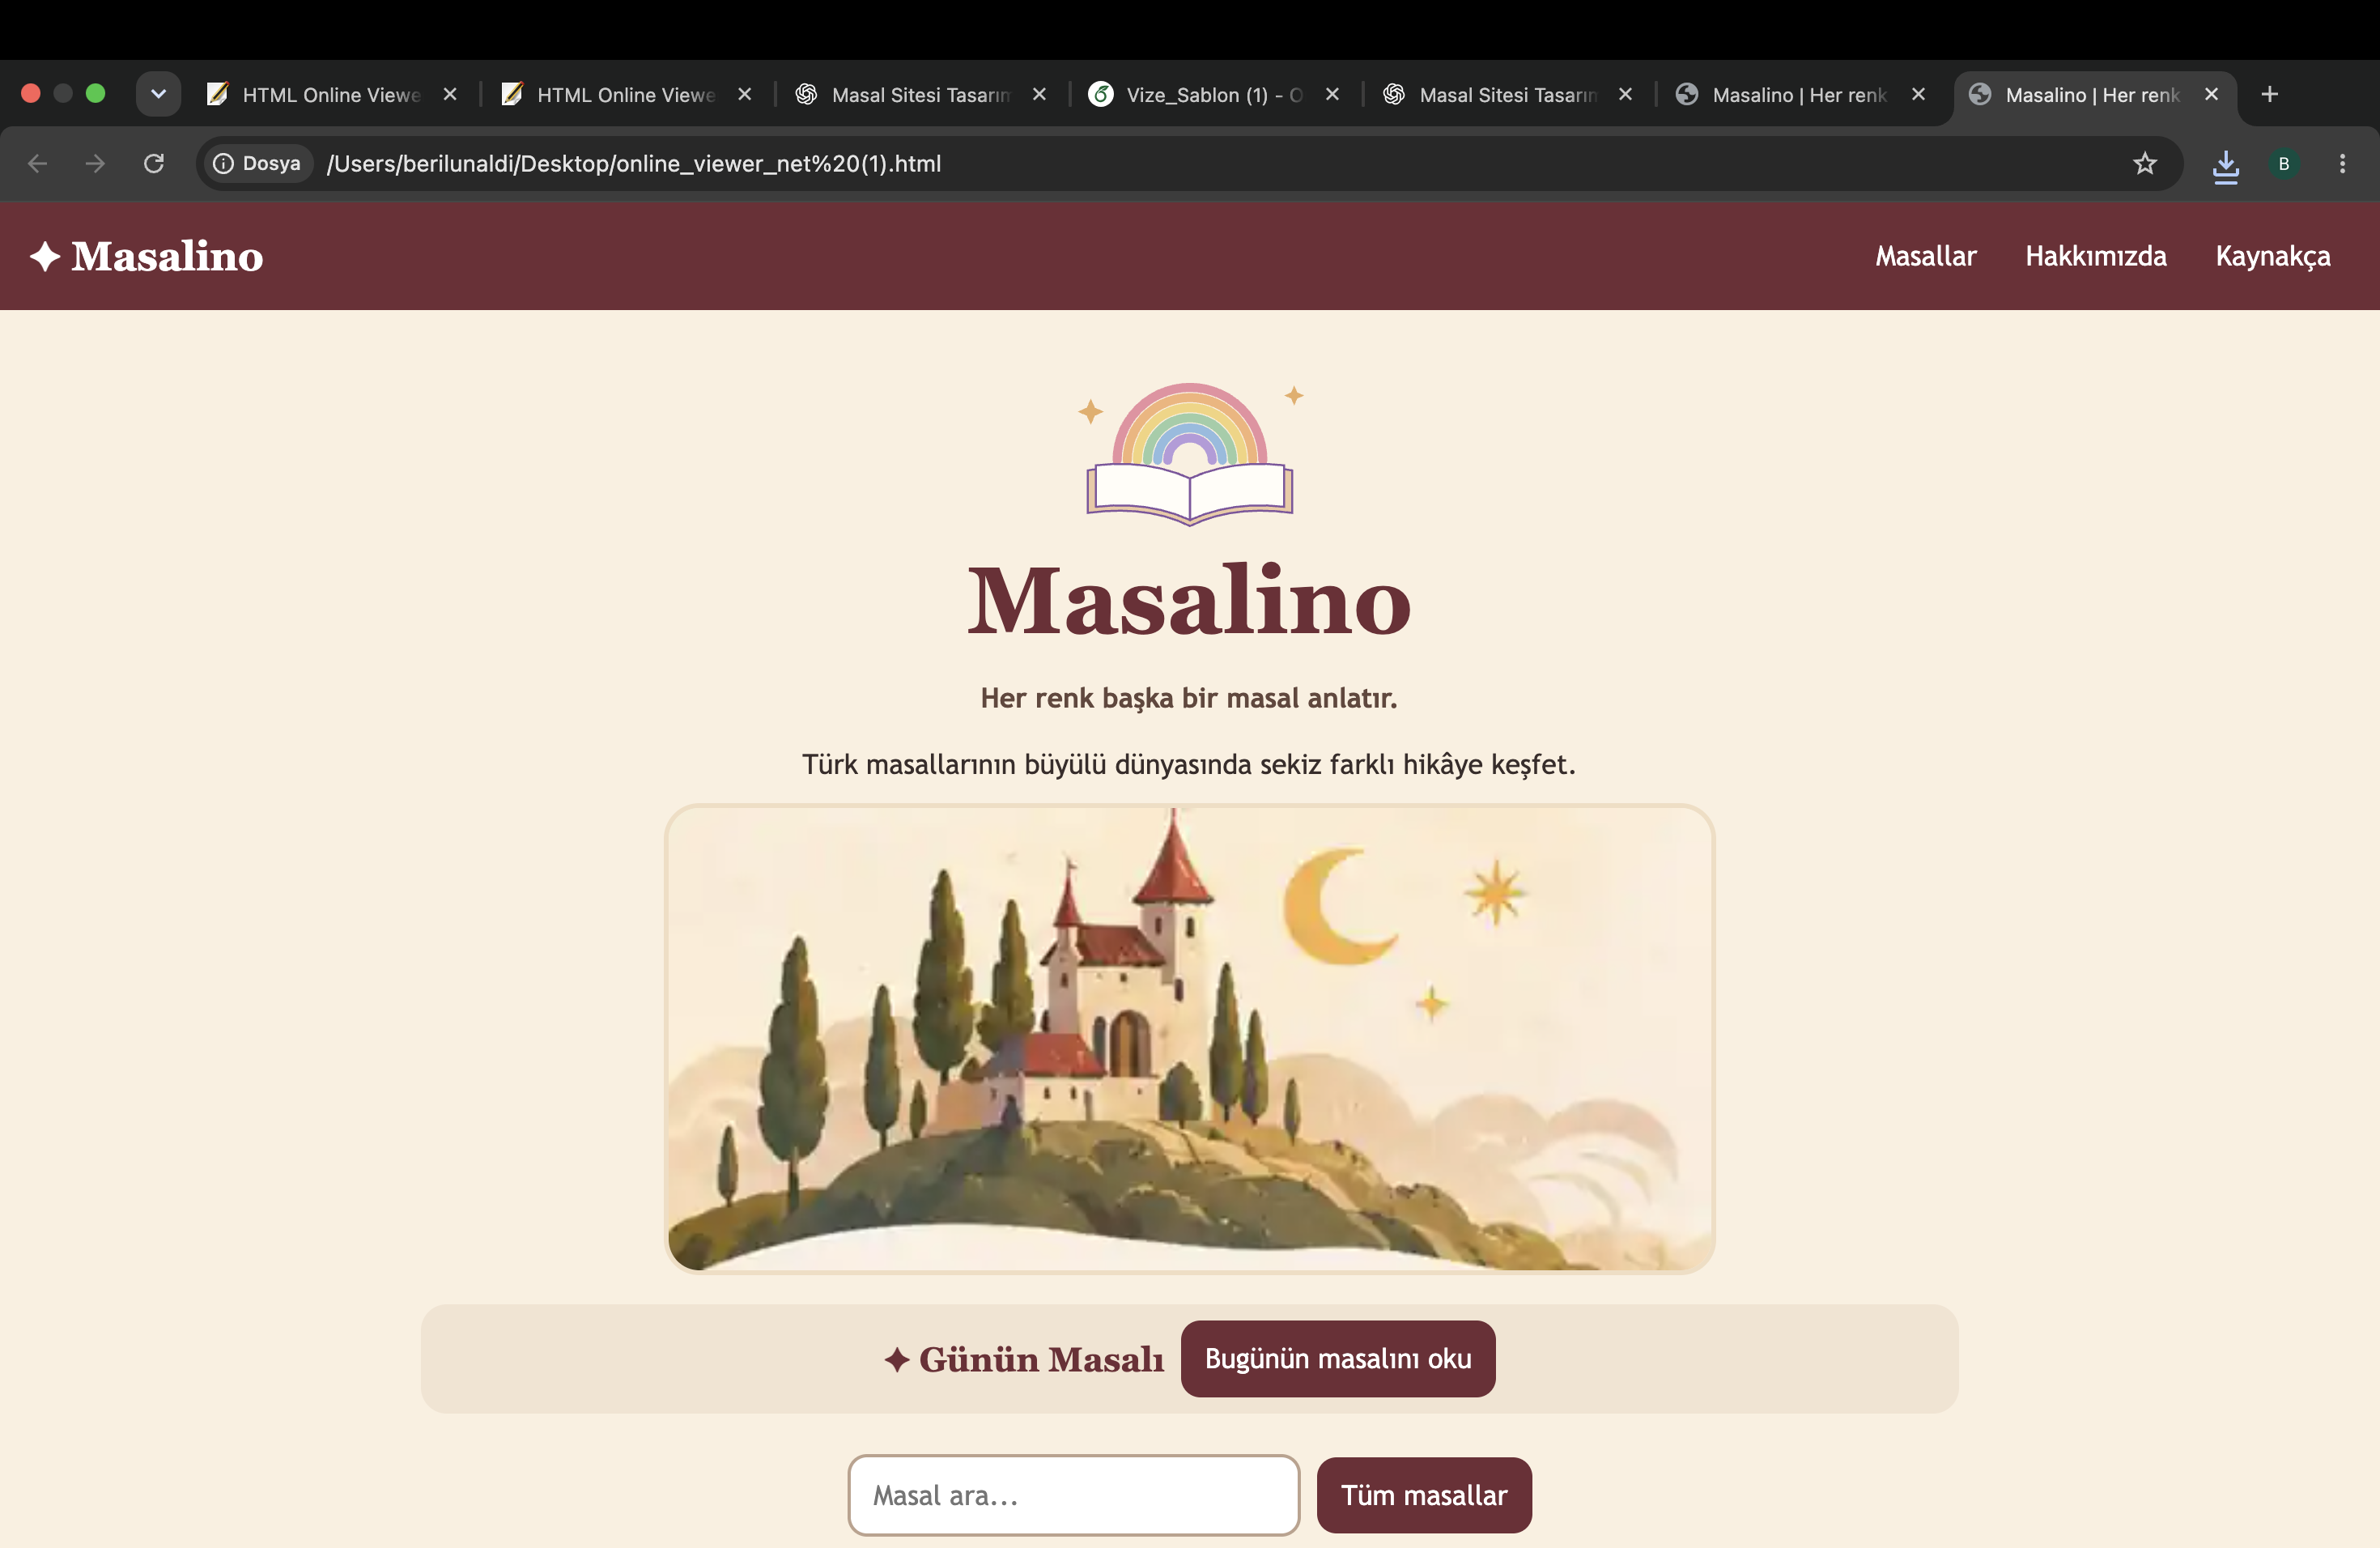
\includegraphics{ekran-masaustu.png}}
  \caption{Sayfanın bilgisayar görünümü}
 \end{figure}
\begin{figure}
  \centering
\resizebox{0.20\textwidth}{!}{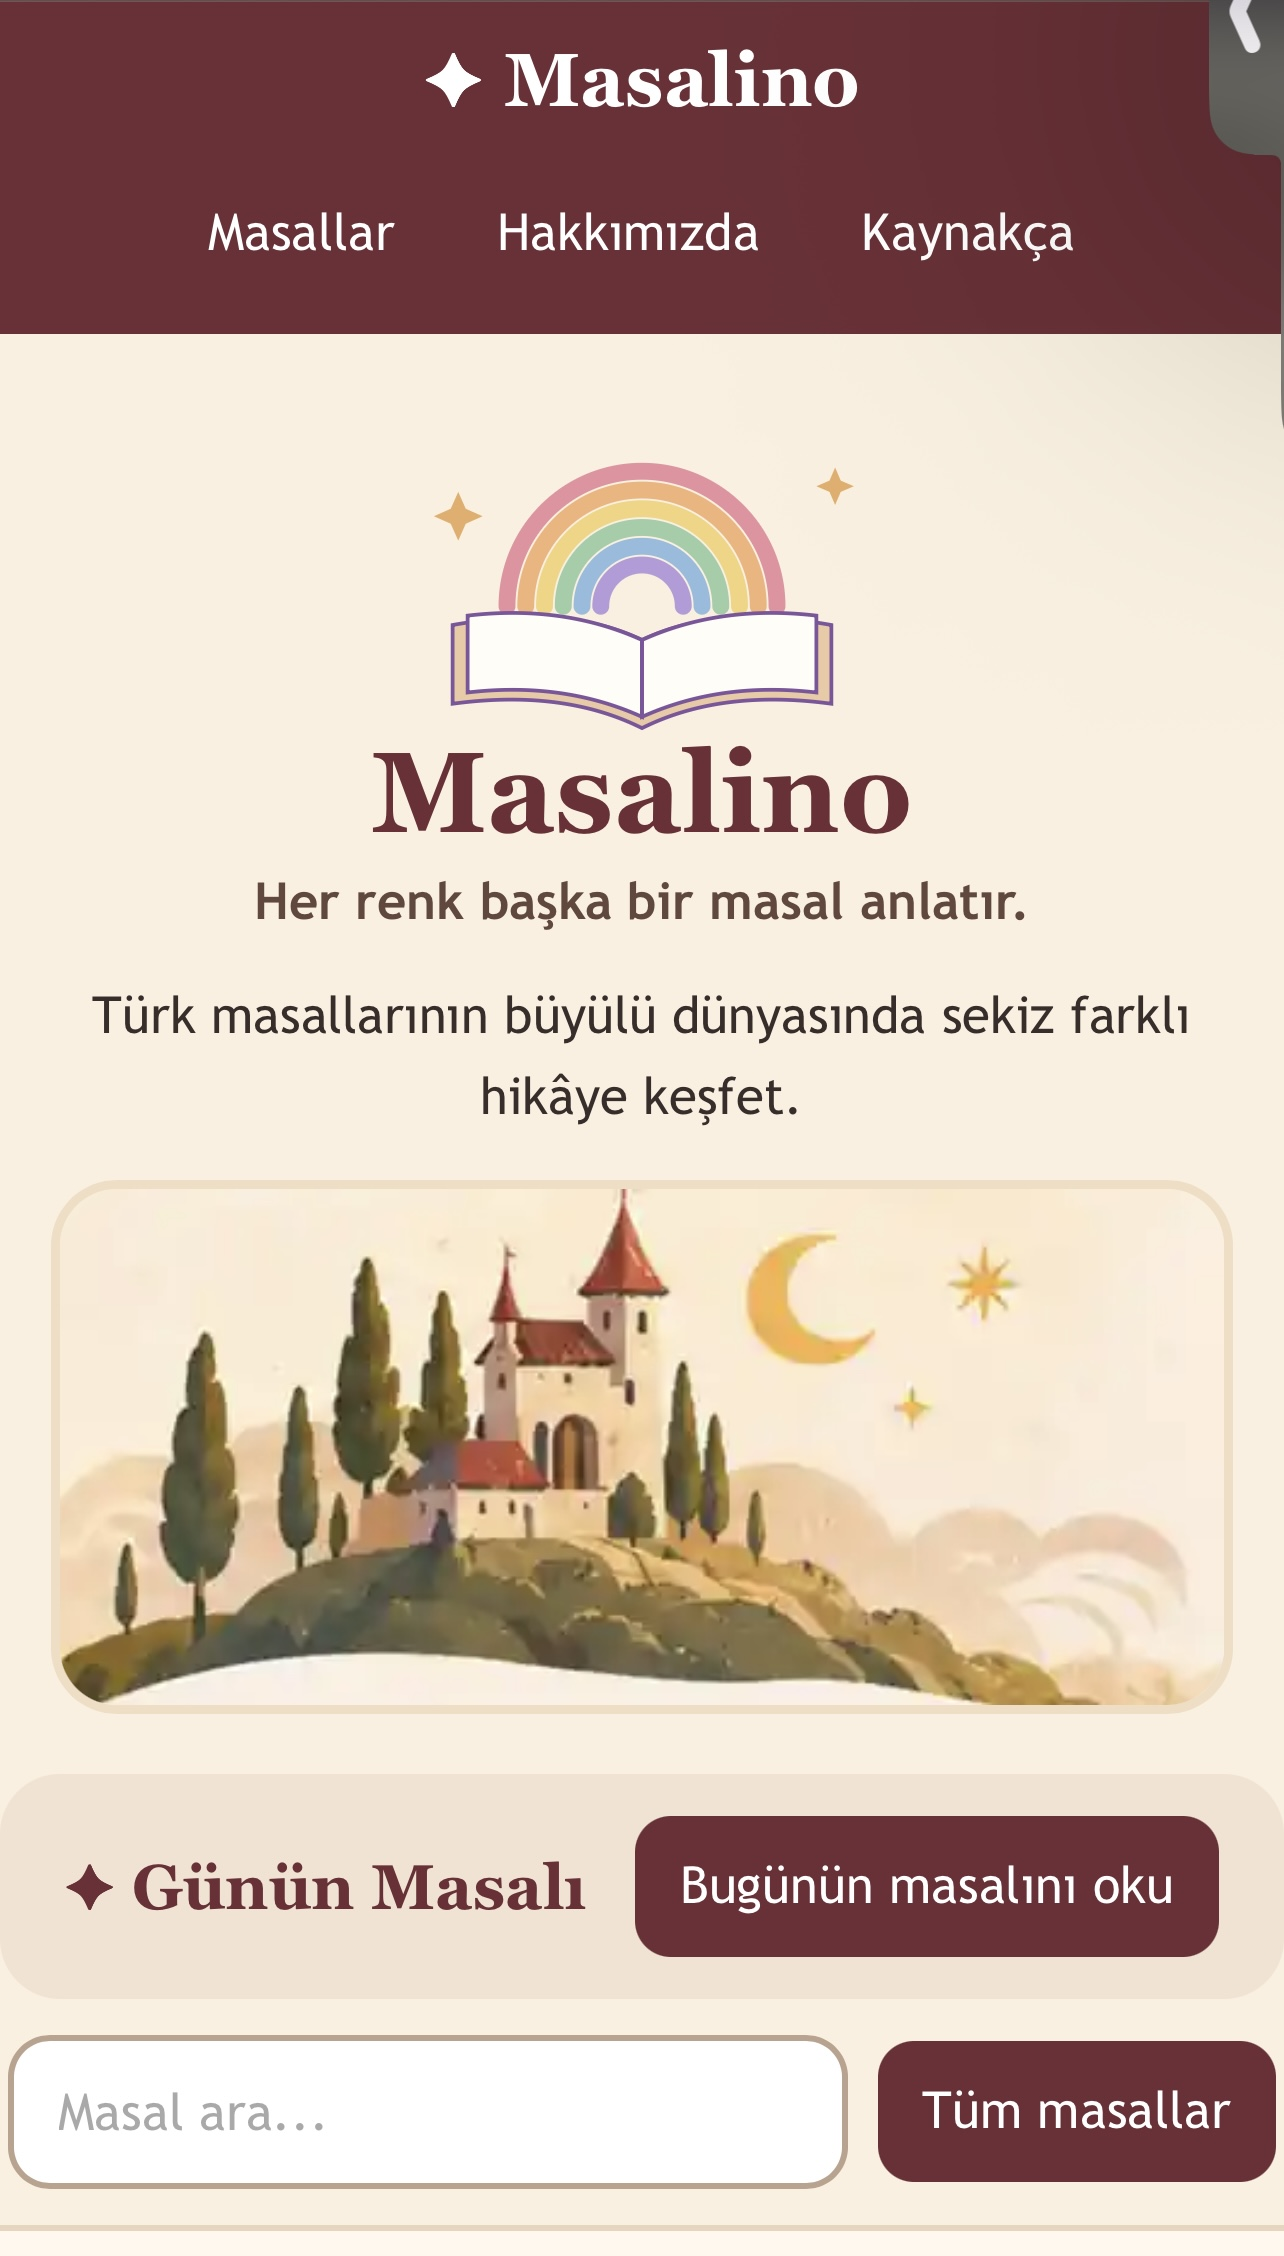
\includegraphics{ekran-mobil.png}}
   \caption{Sayfanın telefon görünümü}
\end{figure}
% ====================================================================
\aciklama{Masalino sitesini HTML, CSS ve JavaScript kullanarak oluşturdum. HTML ile sayfanın temel yapısını hazırladım, CSS ile renkleri, yazı tiplerini ve sayfa düzenini belirledim. JavaScript ile de masal arama, masallar arasında geçiş yapma, yazı boyutunu değiştirme ve farklı okuma seçenekleri gibi özelliklerin çalışmasını sağladım. Bu üç yapıyı bir arada kullanarak hem görsel olarak masal temasına uygun hem de kullanıcıların rahatça gezinebileceği bir site hazırlamayı amaçladım.}

\subsection{HTML Yapısı}
HTML ile sitenin temel yapısını oluşturdum. `<header>` bölümünde Masalino logosuna, site başlığına ve menüye yer verdim. `<main>` içinde masal kartlarını ve hikâyelerin okunduğu alanı düzenledim. Masalları göstermek için `<article>`, farklı bölümleri ayırmak için `<section>` etiketlerini kullandım. Butonları `<button>`, arama alanını ise `<input>` ile oluşturdum. Kaynakları listelemek için `<ul>` ve `<li>` etiketlerinden yararlandım. Sayfanın en altında da `<footer>` ile alt bilgi bölümünü hazırladım.

\subsection{İçsel CSS}
CSS ile sitenin renklerini, yazı tiplerini, kartlarını ve genel sayfa düzenini oluşturdum. Renkleri kolayca yönetebilmek için değişkenler kullandım. Masal kartlarını Grid ile düzenledim, menü ve butonların yerleşiminde ise Flex kullandım. Ayrıca ekran boyutuna göre kartların yerleşimini değiştiren kurallar ekleyerek sitenin telefon ve bilgisayarda düzgün görünmesini sağladım.

\begin{lstlisting}[caption={İçsel CSS'ten önemli bir bölüm}]
  .card {
  border-radius: 16px;
  padding: 20px;
  transition: transform 0.2s;
 
\end{lstlisting}

\subsection{İçsel JavaScript}
Masalino sitesinde masal bilgilerini JavaScript içerisinde bir dizi (array) olarak tuttum. Bu dizide masalların başlıkları, çocuk ve yetişkin anlatımları gibi bilgiler bulunuyor. JavaScript ile arama yapılmasını, günün masalının seçilmesini ve sayfadaki bazı etkileşimlerin çalışmasını sağladım. Kullanıcıların butonlarla gerçekleştirdiği işlemleri de olaylar (events) aracılığıyla düzenledim.

\begin{lstlisting}[caption={İçsel JavaScript'ten önemli bir bölüm}]
 const tales = [
  
const tales = [
    { title: "Nardaniye Hanım" },
    { title: "Fesleğenci Kızı" }
];

function searchTales(query) {
    return tales.filter(tale =>
        tale.title.toLocaleLowerCase("tr")
            .includes(query.toLocaleLowerCase("tr"))
    );
}

  

\end{lstlisting}

\subsection{Sayfanın Özellikleri}


% ====================================================================
\section{Yapay Zekâ Kullanımı}
% ====================================================================
Bu projede yapay zekâdan kod yazma sürecinde ve bazı görsellerin oluşturulmasında destek aldım. Özellikle HTML, CSS ve JavaScript kodlarını hazırlarken ve düzenlerken yapay zekâdan yararlandım. Ancak kodların ne işe yaradığını ve sitenin nasıl çalıştığını anlamaya çalıştım. Tasarımın renklerini, sayfa düzenini ve genel görünümünü kendi tercihlerime göre belirledim. Yapay zekâyı projeyi tamamen hazırlayan bir araç olarak değil, geliştirme sürecinde bana yardımcı olan bir araç olarak kullandım.

\begin{longtable}{@{}p{2.6cm}p{3.6cm}p{4.2cm}p{3.4cm}@{}}
\toprule
\textbf{Araç} & \textbf{Ne için kullandınız?} & \textbf{İstem (prompt) özeti} & \textbf{Sayfada nerede?} \\
\midrule
\endhead
ChatGPT & Kod & HTML, CSS ve JavaScript kodlarını hazırlama ve düzenleme konusunda destek aldım. & Sitenin genelinde \\
ChatGPT & Görsel & Masal temasına uygun kapak görselinin oluşturulmasında destek aldım. & Ana sayfa \\
\bottomrule
\end{longtable}

\subsection{Anladığım ve Kendim Yaptığım Kısımlar}
Yapay zekâdan aldığım kodları kendi tasarım tercihlerime göre düzenledim. Sitenin renklerini, yazı tiplerini, masal kartlarının görünümünü ve sayfa düzenini belirledim. Kodların nasıl çalıştığını anlamak için HTML, CSS ve JavaScript bölümlerini inceledim. Özellikle masalların açılması, arama yapılması ve sayfalar arasında geçiş gibi özelliklerin nasıl çalıştığını öğrendim. Siteyi bilgisayarda ve telefonda açarak kontrol ettim ve karşılaştığım sorunları düzeltmeye çalıştım.

% ====================================================================
\section{Haftalık Katkılar}
% ====================================================================
Her hafta ders içinde yaptığınız çalışmayı kısaca yazın (2--4 cümle). Hangi
özelliği eklediğinizi ya da neyi düzelttiğinizi belirtin ve ilgili commit mesajını
ya da bağlantısını ``Commit'' satırına yazın. Her satıra ekran görüntüsü ekleyin:
resimleri \texttt{hafta1.png}, \texttt{hafta2.png}, \ldots{} adıyla Overleaf
projesine yükleyin. Aynı haftaya ikinci bir görsel eklemek için
\texttt{hafta1b.png} gibi bir dosya yükleyin; kendiliğinden görünür.
Her haftanın altındaki kutulardan o hafta için geçerli olanı $\boxtimes$ ile
işaretleyin: dersin kendisinde katılım gösterdiyseniz ``Ders içinde katılım
sergiledim'', o haftayı sonradan tamamladıysanız ``Telafi yaptım''. Telafi
yaptıysanız yapılan çalışmanın metninde bunu açıkça belirtin.

\begin{longtable}{@{}>{\raggedright\arraybackslash}p{1.7cm}%
                    >{\raggedright\arraybackslash}p{6.4cm}%
                    >{\centering\arraybackslash}p{6cm}@{}}
\toprule
\rowcolor{ana}\textcolor{white}{\textbf{Hafta}} & \textcolor{white}{\textbf{Yapılan çalışma}} & \textcolor{white}{\textbf{Görsel}} \\
\midrule
\endfirsthead
\toprule
\rowcolor{ana}\textcolor{white}{\textbf{Hafta}} & \textcolor{white}{\textbf{Yapılan çalışma}} & \textcolor{white}{\textbf{Görsel}} \\
\midrule
\endhead
\bottomrule
\textbf{1. hafta}\newline 23 Eylül 2026 &
Bu çalışmada temel HTML etiketleri ve CSS kullanılarak bir web sayfası tasarlanmıştır. Ayrıca listeleme ve sayfa içi bağlantılar kullanılarak kullanıcıların içerikler arasında kolayca gezinmesi sağlanmıştır. \newline \textbf{Commit:} Henüz eklenmedi. \newline $\boxtimes$ Ders içinde katılım sergiledim
\newline $\square$ Telafi yaptım & 
\begin{minipage}[t]{\linewidth}
  \vspace{0pt}
  \centering
  \haftagorsel{hafta1.png}\haftaek{hafta1b.png}
\end{minipage} \\
\midrule
\textbf{2. hafta}\newline 30 Eylül 2026 &
Bu hafta HTML ve CSS kullanarak Gossip Girl temalı bir web sayfası üzerinde çalıştım. Sayfaya görseller ve metinler ekleyerek içerikleri düzenledim. Yazıların ve görsellerin yerleşimini ayarlayarak sayfanın görünümünü geliştirdim. \newline \textbf{Commit:} Henüz eklenmedi. \newline $\boxtimes$ Ders içinde katılım sergiledim
\newline $\square$ Telafi yaptım & 
\begin{minipage}[t]{\linewidth}
  \vspace{0pt}
  \centering
  \haftagorsel{hafta2.png}\haftaek{hafta2b.png}
\end{minipage} \\
\midrule
\textbf{3. hafta}\newline 7 Ekim 2026 &
Bu hafta HTML kodları üzerinde çalışarak web sayfasına farklı içerikler ekledim. Sayfanın yapısını düzenledim ve yazdığım kodların ekranda nasıl göründüğünü kontrol ettim. Farklı etiketler kullanarak öğrendiklerimi uyguladım. \newline \textbf{Commit:} Henüz eklenmedi. \newline $\boxtimes$ Ders içinde katılım sergiledim
\newline $\square$ Telafi yaptım & 
\begin{minipage}[t]{\linewidth}
  \vspace{0pt}
  \centering
  \haftagorsel{hafta3.png}\haftaek{hafta3b.png}
\end{minipage} \\
\midrule
\textbf{4. hafta}\newline 14 Ekim 2026 &
Bu hafta JavaScript kullanarak bir hafıza ve eşleştirme oyunu üzerinde çalıştım. Kartlara tıklandığında renklerin açılmasını, eşleşen kartların kaybolmasını ve eşleşmeyen kartların kırmızıya dönmesini sağladım. Ayrıca bağlantı ve yönlendirme işlemleri üzerinde çalışarak butonlara tıklandığında farklı web sitelerine geçiş yapılmasını denedim. \newline \textbf{Commit:} Henüz eklenmedi. \newline $\square$ Telafi yaptım
\newline $\boxtimes$ Ders içinde katılım sergiledim & 
\begin{minipage}[t]{\linewidth}
  \vspace{0pt}
  \centering
  \haftagorsel{hafta4.png}\haftaek{hafta4b.png}
\end{minipage} \\
\midrule
\textbf{5. hafta}\newline 21 Ekim 2026 &
Bu hafta HTML, CSS ve JavaScript kullanarak farklı uygulamalar üzerinde çalıştım. Kodları düzenleyerek sayfaların tasarımlarını oluşturdum, butonlar ve etkileşimli özellikler ekledim. Yaptığım çalışmaları tarayıcıda test ederek kodların nasıl çalıştığını gözlemledim ve gerekli düzenlemeleri yaptım. \newline \textbf{Commit:} Henüz eklenmedi. \newline $\boxtimes$ Ders içinde katılım sergiledim
\newline $\square$ Telafi yaptım & 
\begin{minipage}[t]{\linewidth}
  \vspace{0pt}
  \centering
  \haftagorsel{hafta5.png}\haftaek{hafta5b.png}
\end{minipage} \\
\midrule
\end{longtable}

% ====================================================================
\section{Test ve Değerlendirme}
% ====================================================================
\aciklama{Sayfayı hangi tarayıcı ve cihazlarda denediniz? Çalışmayan bir özellik
olduysa dürüstçe yazın ve nedenini açıklayın.}

\begin{center}
\rowcolors{2}{acik}{white}
\begin{tabular}{@{}p{6cm}p{3.4cm}p{3.4cm}@{}}
\toprule
\rowcolor{ana}\textcolor{white}{\textbf{Özellik}} & \textcolor{white}{\textbf{Bilgisayar}} & \textcolor{white}{\textbf{Telefon}} \\
\midrule
\relax[Masal kartlarının açılması] & [Çalışıyor] & [Çalışıyor] \\
\relax[Masal arama özelliği] & [Çalışıyor] & [Çalışıyor] \\
\relax[Sayfanın ekran boyutuna uyumu] & [Çalışıyor] & [Sorun var] \\
\bottomrule
\end{tabular}
\end{center}

\textbf{Denenen tarayıcılar:} [Chrome, Safari]

% ====================================================================
\section{Sunum Videosu}
% ====================================================================
\begin{center}
\begin{tabular}{@{}ll@{}}
\textbf{Video süresi:} & [dakika:saniye] \quad \aciklama{12--18 dakika olmalıdır} \\
\textbf{Görünürlük:} & [Listelenmemiş / Herkese açık] \\
\textbf{Bağlantı:} & \youtubelink \\
\end{tabular}
\end{center}

\subsection{Video Kontrol Listesi}
\aciklama{Teslimden önce hepsini kontrol edin ve kutuları $\boxtimes$ ile işaretleyin.}
\begin{itemize}[label={}]
  \item $\boxtimes$ Süre 12--18 dakika aralığında.
  \item $\boxtimes$ Sunum boyunca kameram açık, yüzüm görünüyor.
  \item $\boxtimes$ Görünürlük \textbf{Listelenmemiş} (ya da Herkese açık); \textbf{Özel} değil.
  \item $\boxtimes$ Bağlantıyı gizli pencerede açtım, video oynuyor.
  \item $\boxtimes$ YouTube videoyu işlemeyi bitirdi.
  \item $\boxtimes$ Videoyu baştan sona izledim; ses ve kamera tüm sunumda var.
  \item $\boxtimes$ Kapaktaki bağlantı ile bu bölümdeki bağlantı aynı.
\end{itemize}

% ====================================================================
\section{Sonuç ve Kendi Değerlendirmem}
% ====================================================================
\aciklama{Projeden ne öğrendiniz? En çok nerede zorlandınız ve nasıl çözdünüz? İleride
neyi geliştirirdiniz? 6--10 cümle yeterlidir.}

Bu projeyi hazırlarken düşündüğümden çok daha fazla zorlandım ve oldukça fazla zaman harcadım. Özellikle kodları birbirine bağlamak, istediğim tasarımı oluşturmak ve yaptığım değişikliklerin bazen beklediğim gibi sonuçlanmaması kafamı karıştırdı. Bir sorunu çözdüğümde başka bir sorunla karşılaştığım zamanlar oldu. Bazen küçük bir değişiklik yapmak için bile uzun süre uğraşmam gerekti. En çok da sitemin bilgisayarda düzgün görünmesine rağmen telefonda bazı özelliklerinin çalışmaması beni zorladı. Bu süreçte birçok kez kodlarımı yeniden düzenledim, farklı yöntemler denedim ve yapay zekâdan yardım aldım. Zorlandığım yerler olsa da denedikçe kodların nasıl çalıştığını daha iyi anlamaya başladım. Özellikle başlangıçta karmaşık gelen işlemleri zamanla daha rahat yapabildiğimi fark ettim. Genel olarak bu proje benim için yorucu, zaman zaman kafa karıştırıcı ama aynı zamanda birçok yeni şey öğrendiğim bir deneyim oldu.

% ====================================================================
\section{Kaynakça}
% ====================================================================
Masalino web sitesinde yer alan masal metinlerini kendi cümlelerimle hazırladım. Masalların içeriklerini oluştururken Pertev Naili Boratav'ın masal derlemelerinden yararlandım. Web sitesinin tasarımında kullandığım masaüstü görselleri ChatGPT aracılığıyla oluşturuldu. HTML, CSS ve JavaScript kodlarını hazırlarken de yapay zekâ desteğinden yararlandım.



\begin{thebibliography}{9}

\bibitem{boratav}
Boratav, P. N. \emph{Az Gittik Uz Gittik}. Masal derlemesi.

\bibitem{gorseller}
OpenAI. (2026). \emph{Masalino web sitesi için oluşturulan görseller}. ChatGPT.

\end{thebibliography}



% ====================================================================
\appendix
\section{Teslim Kontrol Listesi}
% ====================================================================
\aciklama{Teslim etmeden önce işaretleyin. Bu sayfayı teslim edilen PDF'te bırakabilirsiniz.}
\begin{itemize}[label={}]
  \item $\boxtimes$ MEBİS'e \textbf{yalnızca bu raporun PDF'ini} yükleyeceğim. ZIP ve HTML dosyası yüklemeyeceğim.
  \item $\boxtimes$ PDF dosya adı \texttt{OgrenciNo\_AdSoyad\_vize.pdf} biçiminde.
  \item $\boxtimes$ Kapaktaki GitHub ve YouTube bağlantıları doğru; PDF'te tıklayıp denedim.
  \item $\boxtimes$ GitHub deposunda web sayfası (tek \texttt{.html}), rapor PDF'i, \texttt{.tex} kaynakları ve \texttt{README.md} var.
  \item $\boxtimes$ GitHub deposu \textbf{herkese açık} (ya da öğretim üyesine erişim verdim).
  \item $\boxtimes$ Çalışmamın son hâli teslim saatinden \textbf{önce} depoya gönderildi (sonraki commitler değerlendirilmez).
  \item $\boxtimes$ Sayfa içsel CSS ve içsel JavaScript kullanıyor, harici dosya gerektirmiyor.
  \item $\boxtimes$ Hazır taslak kullanmadım; yapay zekâ kullandıysam Bölüm 5'i doldurdum.
  \item $\boxtimes$ Çalışmanın mantığını sunumda anlatabilirim.
\end{itemize}

\end{document}